% Figure 1 of the RSC proceedings paper (revision 2): the certification pipeline.
% Hand-placed TikZ (no automatic layout). Build:
%   pdflatex -output-directory figures figures/rsc_pipeline.tex
% Drawn at the MDPI full page width (18.4 cm); included with \includegraphics.
\documentclass[border=2pt]{standalone}
\usepackage[T1]{fontenc}
\usepackage{mathpazo}
\usepackage{amsmath,amssymb}
\usepackage{tikz}
\usetikzlibrary{arrows.meta,decorations.pathreplacing,calc}

\definecolor{ink}{HTML}{1F2A36}
\definecolor{model}{HTML}{1F4E79}
\definecolor{good}{HTML}{2E7D32}
\definecolor{bad}{HTML}{C00000}
\definecolor{meas}{HTML}{6B4E16}
\definecolor{soft}{HTML}{5F5F5F}

\begin{document}
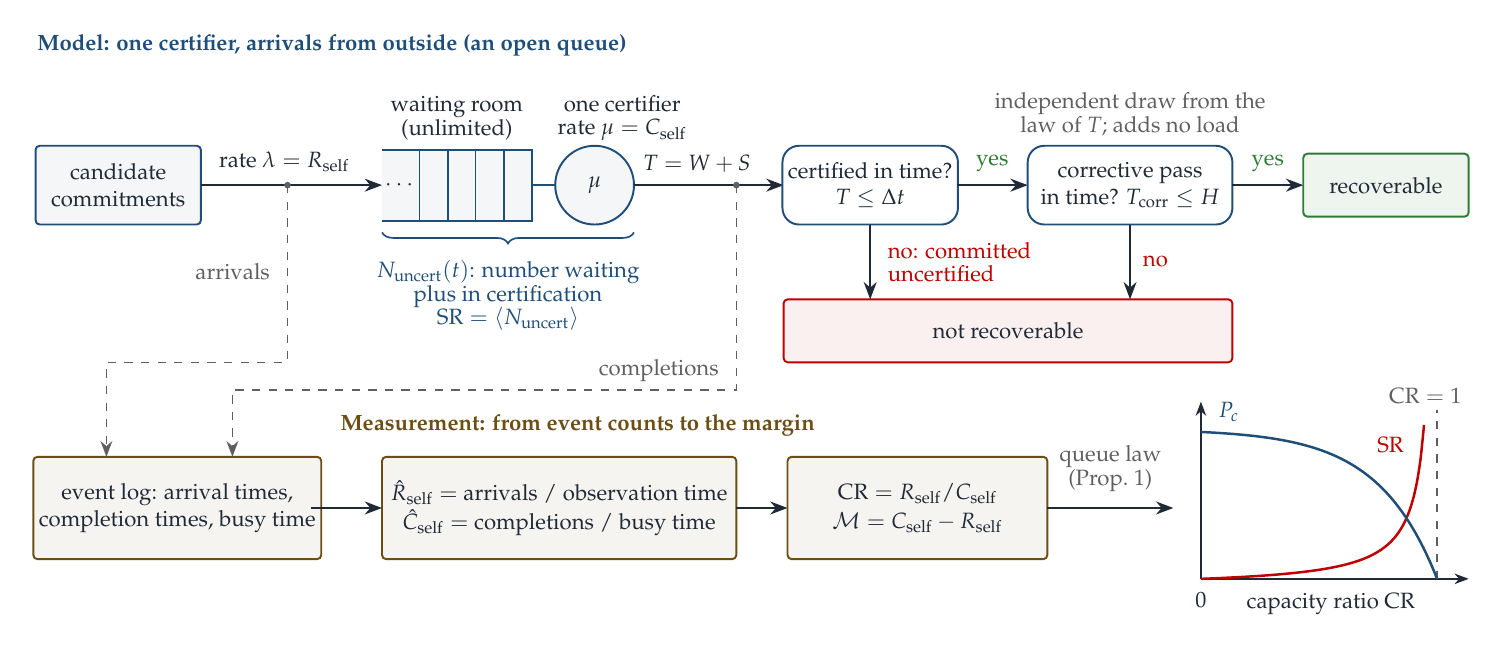
\begin{tikzpicture}[x=1cm,y=1cm,
  font=\footnotesize, text=ink,
  flow/.style={-{Stealth[length=2.2mm]}, line width=0.7pt, draw=ink},
  obs/.style={-{Stealth[length=2mm]}, line width=0.5pt, draw=soft, dashed},
  box/.style={draw=model, line width=0.7pt, rounded corners=1.5pt, fill=model!5,
              align=center, inner sep=2pt},
  test/.style={draw=model, line width=0.7pt, rounded corners=6pt, fill=white,
               align=center, inner sep=2pt},
  mbox/.style={draw=meas, line width=0.7pt, rounded corners=1.5pt, fill=meas!6,
               align=center, inner sep=2pt},
  lane/.style={font=\footnotesize\bfseries, anchor=west}]

\path[use as bounding box] (0,0.05) rectangle (18.4,7.6);

% ------------------------------------------------------------------ model lane
\node[lane, text=model] at (0,7.38)
  {Model: one certifier, arrivals from outside (an open queue)};

\node[box, minimum width=2.1cm, minimum height=1.0cm] at (1.15,5.6)
  {candidate\\commitments};
\draw[flow] (2.2,5.6) -- (4.5,5.6)
  node[pos=0.46, above=1pt] {rate $\lambda=R_{\mathrm{self}}$};

% waiting room: open on the arrival side
\draw[draw=model, line width=0.7pt, fill=model!5]
  (4.5,6.05) -- (6.4,6.05) -- (6.4,5.15) -- (4.5,5.15);
\foreach \x in {4.98,5.34,5.69,6.05} {\draw[draw=model, line width=0.5pt] (\x,6.05) -- (\x,5.15);}
\node at (4.74,5.6) {$\cdots$};
\node[align=center] at (5.45,6.45) {waiting room\\[-1pt](unlimited)};

% certifier
\draw[draw=model, line width=0.7pt] (6.4,5.6) -- (6.7,5.6);
\draw[draw=model, line width=0.7pt, fill=model!5] (7.2,5.6) circle (0.5);
\node at (7.2,5.6) {$\mu$};
\node[align=center] at (7.55,6.45) {one certifier\\[-1pt]rate $\mu=C_{\mathrm{self}}$};

% N_uncert = queue + server
\draw[decorate, decoration={brace, mirror, amplitude=4pt}, line width=0.6pt, draw=model]
  (4.5,5.0) -- (7.7,5.0);
\node[align=center, text=model] at (6.1,4.2)
  {$N_{\mathrm{uncert}}(t)$: number waiting\\[-1pt]plus in certification\\[-1pt]
   $\mathrm{SR}=\langle N_{\mathrm{uncert}}\rangle$};

% sojourn -> deadline test
\draw[flow] (7.7,5.6) -- (9.6,5.6)
  node[pos=0.42, above=1pt] {$T=W+S$};
\node[test, minimum width=2.2cm, minimum height=1.0cm] at (10.7,5.6)
  {certified in time?\\$T\le\Delta t$};
\draw[flow] (11.8,5.6) -- (12.7,5.6) node[midway, above=1pt, text=good] {yes};
\node[test, minimum width=2.6cm, minimum height=1.0cm] at (14.0,5.6)
  {corrective pass\\in time? $T_{\mathrm{corr}}\le H$};
\node[text=soft, align=center] at (14.0,6.5)
  {independent draw from the\\[-1pt]law of $T$; adds no load};
\draw[flow] (15.3,5.6) -- (16.2,5.6) node[midway, above=1pt, text=good] {yes};
\node[box, draw=good, fill=good!8, minimum width=2.1cm, minimum height=0.8cm]
  at (17.25,5.6) {recoverable};

% "no" branches: one outcome box, no crossings
\node[box, draw=bad, fill=bad!6, minimum width=5.7cm, minimum height=0.8cm]
  at (12.45,3.75) {not recoverable};
\draw[flow] (10.7,5.1) -- (10.7,4.15);
\node[text=bad, align=left, anchor=west] at (10.8,4.62) {no: committed\\[-1pt]uncertified};
\draw[flow] (14.0,5.1) -- (14.0,4.15) node[midway, right=1pt, text=bad] {no};

% ------------------------------------------------------------ measurement lane
\node[lane, text=meas] at (3.85,2.55) {Measurement: from event counts to the margin};

\node[mbox, minimum width=3.4cm, minimum height=1.3cm] at (1.9,1.5)
  {event log: arrival times,\\completion times, busy time};
\node[mbox, minimum width=4.5cm, minimum height=1.3cm] at (6.75,1.5)
  {$\hat R_{\mathrm{self}}=$ arrivals $/$ observation time\\[1pt]
   $\hat C_{\mathrm{self}}=$ completions $/$ busy time};
\node[mbox, minimum width=3.3cm, minimum height=1.3cm] at (11.3,1.5)
  {$\mathrm{CR}=R_{\mathrm{self}}/C_{\mathrm{self}}$\\[1pt]
   $\mathcal{M}=C_{\mathrm{self}}-R_{\mathrm{self}}$};
\draw[flow] (3.6,1.5) -- (4.5,1.5);
\draw[flow] (9.0,1.5) -- (9.65,1.5);
\draw[flow] (12.95,1.5) -- (14.55,1.5);
\node[align=center, text=soft] at (13.75,2.0) {queue law\\[-1pt](Prop.~1)};

% what is observed (dashed; the two paths do not cross)
\draw[obs] (3.3,5.6) -- (3.3,3.35) -- (1.0,3.35) -- (1.0,2.15);
\draw[obs] (9.0,5.6) -- (9.0,3.0) -- (2.6,3.0) -- (2.6,2.15);
\fill[soft] (3.3,5.6) circle (1.2pt);
\fill[soft] (9.0,5.6) circle (1.2pt);
\node[text=soft, anchor=east] at (3.2,4.5) {arrivals};
\node[text=soft, anchor=east] at (8.9,3.25) {completions};

% inset: continuous approach to CR = 1 (M/M/1 curves, mu*Dt = 4)
\draw[line width=0.5pt, draw=ink, -{Stealth[length=1.8mm]}] (14.9,0.6) -- (18.3,0.6);
\draw[line width=0.5pt, draw=ink, -{Stealth[length=1.8mm]}] (14.9,0.6) -- (14.9,2.85);
\draw[line width=0.5pt, draw=soft, dashed] (17.9,0.6) -- (17.9,2.75);
\node[text=soft, anchor=south] at (17.75,2.7) {$\mathrm{CR}=1$};
\node[anchor=north] at (16.55,0.55) {capacity ratio $\mathrm{CR}$};
\node[anchor=north] at (14.9,0.55) {$0$};
\draw[line width=0.9pt, draw=bad, domain=0:0.945, samples=70, smooth, variable=\t]
  plot ({14.9+3.0*\t},{0.6+0.115*\t/(1-\t)});
\draw[line width=0.9pt, draw=model, domain=0:1, samples=70, smooth, variable=\t]
  plot ({14.9+3.0*\t},{0.6+1.9*(1-exp(-4*(1-\t)))});
\node[text=bad, anchor=east] at (17.6,2.3) {$\mathrm{SR}$};
\node[text=model, anchor=west] at (15.0,2.72) {$P_c$};
\end{tikzpicture}
\end{document}
